\section{Results}

\subsection{Overall Performance}
Table~\ref{tab:overall} presents overall accuracy by system.
FAISS leads at 75.6\%, followed closely by Naive RAG (74.0\%) and BM25 (73.4\%).
Bootstrap 95\% CIs overlap substantially among the top three, and pairwise McNemar's tests show no significant differences ($p{>}0.3$).
Simple KG (67.2\%) and ChromaDB (41.2\%) are significantly worse ($p{<}0.01$ and $p{<}0.001$ respectively).
ChromaDB uses a different default embedding model (all-MiniLM-L6-v2) than the other vector-based systems; we include it for completeness but note this confound.

\begin{table}[t]
\centering
\resizebox{\columnwidth}{!}{%
\begin{tabular}{lcccc}
\toprule
\textbf{System} & \textbf{Accuracy} & \textbf{95\% CI} & \textbf{F1} & \textbf{Ver.\ Recall} \\
\midrule
FAISS & \textbf{75.6\%} & [70.8, 80.2] & \textbf{0.870} & \textbf{79.5\%} \\
Naive RAG & 74.0\% & [69.2, 78.9] & 0.867 & 74.4\% \\
BM25 & 73.4\% & [68.2, 78.2] & 0.867 & 69.2\% \\
Simple KG & 67.2\% & [61.7, 72.4] & 0.841 & 75.6\% \\
ChromaDB$^{\dagger}$ & 41.2\% & [35.7, 46.8] & 0.744 & 37.2\% \\
\bottomrule
\end{tabular}%
}
\caption{Overall results on BiTempQA (308 questions). $^{\dagger}$\ ChromaDB uses a different embedding model (see \S\ref{sec:limitations}).}
\label{tab:overall}
\end{table}

\subsection{Record-Time Reasoning Is Genuinely Harder}

\begin{table}[t]
\centering
\resizebox{\columnwidth}{!}{%
\begin{tabular}{lcccc}
\toprule
\textbf{System} & \textbf{Event-Only (110Q)} & \textbf{Record-Only (24Q)} & \textbf{Both Req. (174Q)} & \textbf{Ver.\ Track. (78Q)} \\
\midrule
FAISS & 79.1\% & 66.7\% & \textbf{74.7\%} & \textbf{79.5\%} \\
Naive RAG & 78.2\% & 62.5\% & 73.0\% & 74.4\% \\
BM25 & 77.3\% & 66.7\% & 71.8\% & 69.2\% \\
Simple KG & 66.4\% & 58.3\% & 69.0\% & 75.6\% \\
ChromaDB & 44.5\% & 50.0\% & 37.9\% & 37.2\% \\
\midrule
\textbf{Average} & \textbf{69.1\%} & 60.8\% & 65.3\% & 67.2\% \\
\bottomrule
\end{tabular}%
}
\caption{Accuracy by temporal requirement. Record-only questions (n=24) are hardest across all systems; the gap is suggestive given the small sample size.}
\label{tab:temporal_breakdown}
\end{table}

Table~\ref{tab:temporal_breakdown} shows accuracy by temporal requirement.
Record-only questions average 60.8\% vs.\ 69.1\% for event-only, an 8.3pp gap consistent across all five systems.
To confirm this is not a distribution artifact, we fit a mixed-effects logistic regression with scenario random intercepts, controlling for system identity, question type, difficulty level, and all temporal requirement flags.

\begin{table}[t]
\centering
\small
\begin{tabular}{lccc}
\toprule
\textbf{Predictor} & \textbf{Coef.} & \textbf{z} & \textbf{p} \\
\midrule
\multicolumn{4}{l}{\textit{System effects} (ref: FAISS)} \\
\quad ChromaDB & $-$0.344 & $-$10.53 & $<$0.001 \\
\quad Simple KG & $-$0.084 & $-$2.58 & 0.010 \\
\quad BM25 & $-$0.023 & $-$0.70 & 0.487 \\
\quad Naive RAG & $-$0.016 & $-$0.50 & 0.619 \\
\midrule
\multicolumn{4}{l}{\textit{Temporal requirements}} \\
\quad Record-time required & $-$0.079 & $-$2.26 & \textbf{0.023} \\
\quad Event-time required & 0.061 & 1.08 & 0.280 \\
\quad Version tracking & 0.050 & 1.29 & 0.199 \\
\quad Knowledge retraction & $-$0.080 & $-$1.50 & 0.135 \\
\midrule
Scenario variance & \multicolumn{3}{c}{$\sigma^2{=}0.049$} \\
\bottomrule
\end{tabular}
\caption{Mixed-effects logistic regression (scenario random intercepts, $N{=}1{,}540$). Record-time requirement is the only temporal factor reaching significance.}
\label{tab:regression}
\end{table}

The record-time coefficient ($\beta{=}{-}0.079$, $p{=}0.023$) remains significant after controlling for all confounds (Table~\ref{tab:regression}), confirming that the dual-timestamp dimension captures a genuinely harder reasoning capability.
Notably, difficulty levels (L2/L3) are \emph{not} independently predictive after controls ($p{=}0.103$, $p{=}0.278$), suggesting the difficulty gradient is largely mediated by the distribution of harder question types at higher levels.

\subsection{Per-Question-Type Analysis}

\begin{figure}[t]
\centering
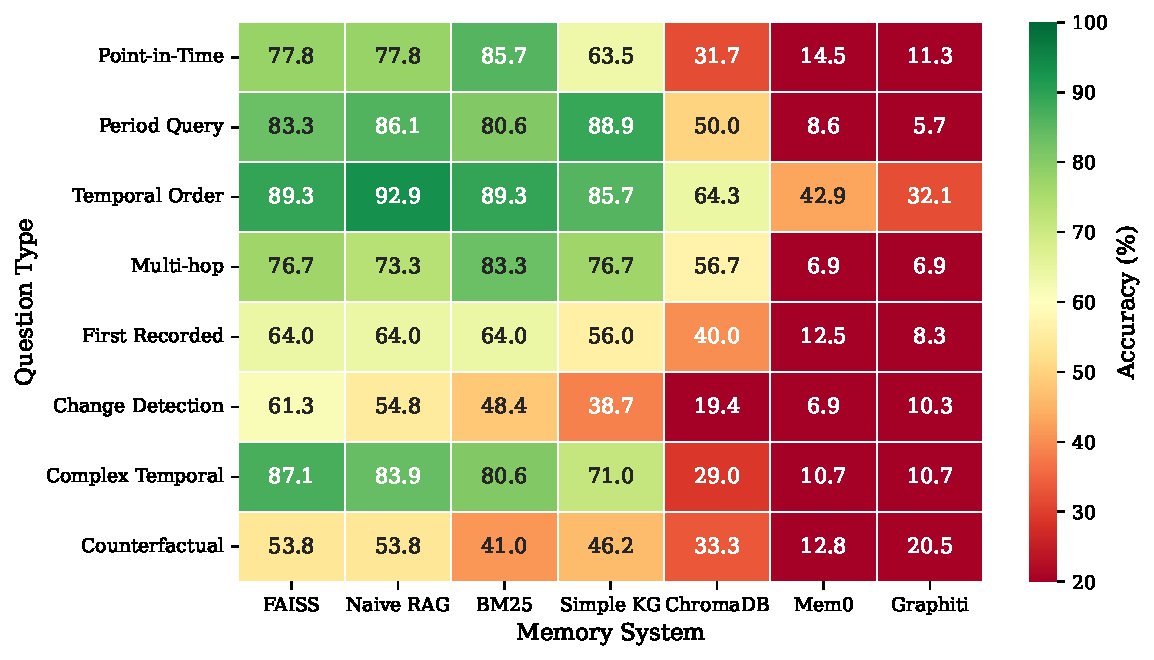
\includegraphics[width=\columnwidth]{figures/fig3_heatmap.pdf}
\caption{System $\times$ question type accuracy heatmap. No single system dominates all types; the 40.6pp spread across types confirms the typology captures distinct challenges.}
\label{fig:heatmap}
\end{figure}

Figure~\ref{fig:heatmap} reveals substantial system$\times$type interactions.
FAISS leads on complex temporal (87.1\%) and counterfactual (53.8\%); BM25 excels at point-in-time (85.7\%) and multi-hop (83.3\%); Simple KG tops period query (88.9\%).
The 40.6pp spread across question types (counterfactual: 48.7\% to temporal order: 89.3\%) validates the typology.

\subsection{Difficulty Calibration}
All five systems show monotonic L1$\to$L3 degradation, but with strikingly different robustness: FAISS drops only 2.9pp vs.\ BM25's 16.6pp (Figure~\ref{fig:difficulty}).
FAISS's dense representations appear to maintain semantic relevance even under complex compositional demands, while BM25's keyword matching deteriorates sharply when query--document lexical overlap decreases.

\begin{figure}[t]
\centering
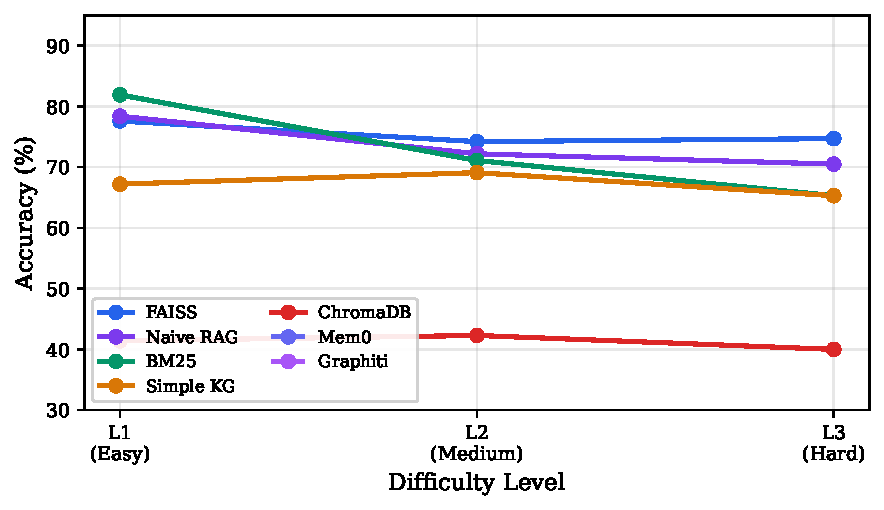
\includegraphics[width=\columnwidth]{figures/fig4_difficulty.pdf}
\caption{Accuracy degradation from L1 to L3. FAISS is most robust ($-$2.9pp); BM25 is most fragile ($-$16.6pp).}
\label{fig:difficulty}
\end{figure}

\subsection{System Complementarity}
An oracle ensemble (correct if \emph{any} system answers correctly) achieves \textbf{85.4\%}, a 9.8pp gain over the best single system, confirming that memory backends have substantially non-overlapping error profiles (Figure~\ref{fig:complementarity}).
FAISS-ChromaDB Jaccard overlap is only 0.446 (lowest), while FAISS-SimpleKG is 0.746.
Simple KG uniquely solves 6 items that FAISS misses, and ChromaDB uniquely solves 6, despite its low overall accuracy.
45 items (14.6\%) are answered incorrectly by \emph{all} systems, establishing a hard irreducible ceiling.

\begin{figure}[t]
\centering
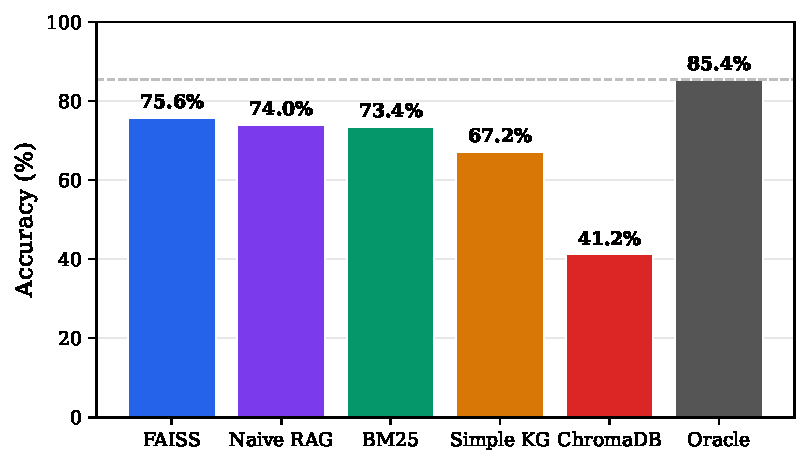
\includegraphics[width=\columnwidth]{figures/fig5_complementarity.pdf}
\caption{Oracle ensemble reaches 85.4\% vs.\ 75.6\% best single system. 45 irreducible failures suggest retrieval-independent challenges.}
\label{fig:complementarity}
\end{figure}

\subsection{Cross-Benchmark Validation with LoCoMo}
Table~\ref{tab:locomo} compares BiTempQA results with LoCoMo evaluation.
The most striking finding is Simple KG's asymmetry: 97.5\% adversarial accuracy on LoCoMo (best of all systems, +34pp above average) but 37.5\% temporal reasoning on LoCoMo (worst, $-$9pp) and 67.2\% on BiTempQA.
This reflects a fundamental trade-off: graph structures resist adversarial hallucination (returning empty context for non-existent facts) but lack the retrieval breadth needed for temporal reasoning.

\begin{table}[t]
\centering
\resizebox{\columnwidth}{!}{%
\begin{tabular}{lccccc}
\toprule
& \multicolumn{2}{c}{\textbf{BiTempQA}} & \multicolumn{3}{c}{\textbf{LoCoMo}} \\
\cmidrule(lr){2-3} \cmidrule(lr){4-6}
\textbf{System} & Overall & Temporal & Overall & Temporal & Adversarial \\
\midrule
FAISS & \textbf{75.6\%} & \textbf{75.6\%} & \textbf{57.0\%} & \textbf{46.9\%} & 63.0\% \\
Naive RAG & 74.0\% & 74.0\% & 54.4\% & 42.7\% & 69.7\% \\
BM25 & 73.4\% & 73.4\% & 55.8\% & 43.8\% & 64.8\% \\
Simple KG & 67.2\% & 67.2\% & 56.8\% & 37.5\% & \textbf{97.5\%} \\
\bottomrule
\end{tabular}%
}
\caption{Cross-benchmark comparison. Simple KG shows extreme adversarial-temporal asymmetry.}
\label{tab:locomo}
\end{table}
